\documentclass[a4paper]{article}

\usepackage{polski}
\usepackage[utf8]{inputenc}

\usepackage{scrextend}
\usepackage{amsfonts}
\usepackage{amsmath}
\usepackage{svg}

\usepackage{geometry}
\geometry{a4paper, left=15mm, top=30mm, right=15mm}

\usepackage{graphicx} 
\usepackage{isotope}
\usepackage{array}
\usepackage{float}

\usepackage{hyperref}
\hypersetup{
    colorlinks,
    citecolor=black,
    filecolor=black,
    linkcolor=black,
    urlcolor=black
}

\date{}

\newenvironment{definition}[1][title]
    {
        \begin{center}
        \begin{tabular}{|p{1\textwidth}|}
        \hline
            Definicja: #1\\[2ex]
        \begin{em}
        \Large
    }
    { 
        \end{em}
        \\\hline
        \end{tabular} 
        \end{center}
    }
    
\begin{document}
    \linespread{1.5}
    \begin{titlepage}
        \centering
        \vspace*{\fill}

        \vspace*{0.5cm}

        \huge\bfseries
        Notatki z wykładów z Fizyki 1

        \vspace*{0.5cm}

        \large Łukasz Kwinta

        \vspace*{\fill}
    \end{titlepage}
    
\pagebreak
\tableofcontents
\pagebreak

\section{\huge Wiadomości wstępne i wektory}
    \Large
    W całych notatkach mogą pojawić się poniżej zdefiniowane wektory - a dokładniej 
    wersory rozpinające przestrzenie $\mathbb{R}^2$ i $\mathbb{R}^3$:\\
    $\mathbb{R}^2$:
    \begin{itemize}
        \item [] $\hat{i} = (1,\ 0)$
        \item [] $\hat{j} = (0,\ 1)$
    \end{itemize}
    $\mathbb{R}^3$:
    \begin{itemize}
        \item [] $\hat{i} = (1,\ 0,\ 0)$
        \item [] $\hat{j} = (0,\ 1,\ 0)$
        \item [] $\hat{k} = (0,\ 0,\ 1)$
    \end{itemize}

    \subsection{\LARGE Suma wektorów}
        \Large 
        Niech:
        \[\vec{a} := (a_1, a_2, a_3) \hspace{1cm} \vec{b} = (b_1, b_2, b_3) \]
        Wtedy suma wektorów ma następującą postać:
        \[\vec{a} + \vec{b} = (a_1 + b_1,\ a_2 + b_2,\ a_3 + b_3)\] \\
        \begin{center}
            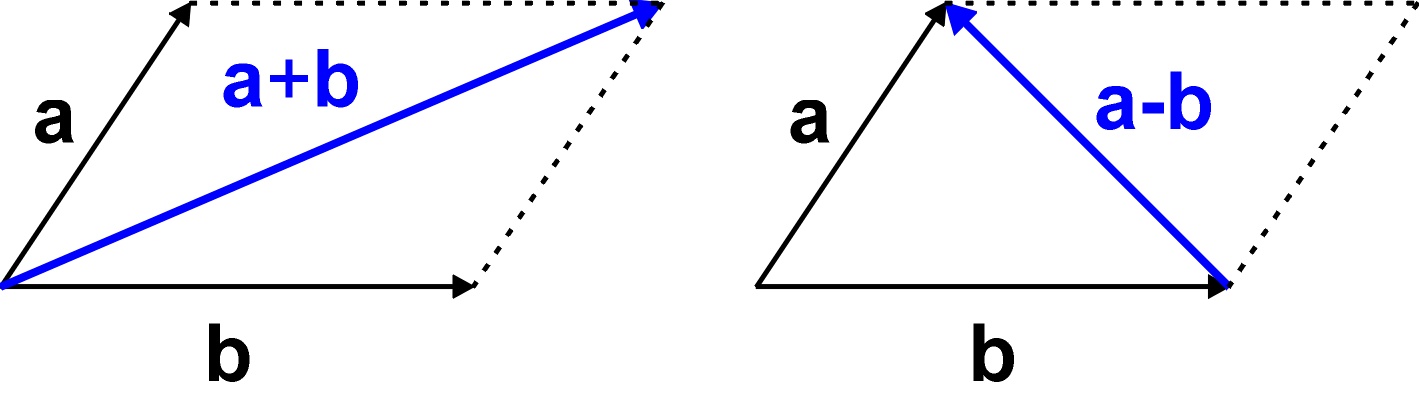
\includegraphics[width=10cm]{img/suma_wektorow.png} 
        \end{center}
        
    \subsection{\LARGE Iloczyn skalarny}
        \Large 
        Niech:
        \[\vec{a} := (a_1, a_2, a_3) \hspace{1cm} \vec{b} = (b_1, b_2, b_3) \]
        Wtedy iloczyn skalarny oznaczamy $\circ$ ma następującą postać:
        \[\vec{a} \circ \vec{b} = a_1 \cdot b_1 + a_2 \cdot b_2 + a_3 \cdot b_3\]
        Występuje również poniższa zależność:
         \[\vec{a} \circ \vec{b} = ||\vec{a}|| \cdot ||\vec{b}|| \cdot \cos{(\ \vec{a},\ {\vec{b}}\ )} \]
        
    \subsection{\LARGE Iloczyn wektorowy}
        \Large 
        Niech:
        \[\vec{a} := (a_1, a_2, a_3) \hspace{1cm} \vec{b} = (b_1, b_2, b_3) \]
        oraz:      
        \[\hat{i} := (1, 0, 0) \hspace{0,75cm} \hat{j} = (0, 1, 0) \hspace{0,75cm} \hat{k} = (0, 0, 1) \]
        Wtedy, iloczyn wektorowy ma następującą postać:
        \[
            \vec{a} \times \vec{b} = 
            \begin{vmatrix}
                \hat{i} & \hat{j} & \hat{k} \\
                a_1 & a_2 & a_3 \\
                b_1 & b_2 & b_3
            \end{vmatrix}
            = \hat{i}(a_2b_3 - a_3b_2) + \hat{j}(a_3b_1 - a_1b3) + \hat{k}(a_1b_2 - a_2b_1) =     
        \]
        \[ = (a_2b_3 - a_3b_2, a_3b_1 - a_1b3, a_1b_2 - a_2b_1 )\]
        Tak jak przy iloczynie skalarnym występuje zależność związana z kątem między wektorami:
        \[||\vec{a} \times \vec{b}|| = ||\vec{a}||\cdot ||\vec{b}|| \cdot \sin{(\ \vec{a},\ {\vec{b}}\ )}\]
        Kierunek iloczynu wektorowego $\vec{a} \times \vec{b}$ jest prostopadły do płaszczyzny 
        stworzonej przez wektory $\vec{a}$ i $\vec{b}$.\\ Natomiast zwrot tego wektora można określić stosując zasadę prawej dłoni: \\
        \begin{center}
            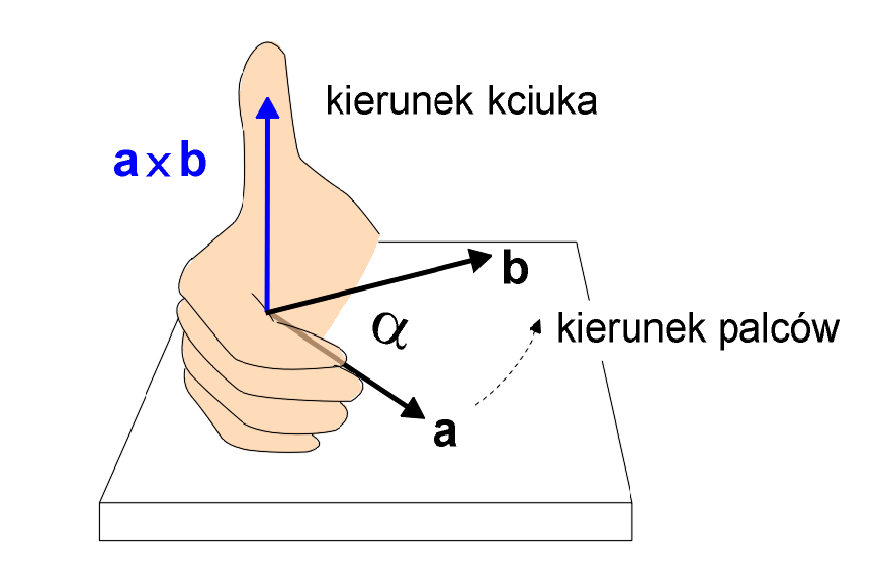
\includegraphics[width=10cm]{img/prawareka.png} 
        \end{center}
        
\section{\huge Podstawy kinematyki}
    \subsection{\LARGE Podstawowe pojęcia}
        \Large
        \begin{definition}[Ruch]
            Zmiana wzajemnego położenia ciał względem innych ciał wraz z upływem czasu.
        \end{definition}
        \begin{definition}[Układ odniesienia]
            Wybrane ciało lub ciało względem których wyznaczamy własności fizyczne takie jak położenie czy prędkość.
        \end{definition}
        \begin{definition}[Punkt materialny]
            Punktem materialnym nazywamy obiekt obdarzony masą, których rozmiar (aka objętość) można zaniedbać.
        \end{definition}
        \begin{definition}[Przemieszczenie]
            Zmiana położenia ciała względem jakiegoś układu odniesienia, zwykle punktu $(0,\ 0)$ w układzie współrzednych. 
            Wektor przemieszczenia oznaczamy $r$. Występuje poniższa zależność:
            \[\vec{r} = \hat{i}x + \hat{j}y + \hat{k}z = (x,\ y,\ z)\]
            gdzie:
            \begin{itemize}
                \item[--] x - współrzedna $x$ wektora przemieszczenia
                \item[--] y - współrzędna $y$ wektora przemieszczenia
                \item[--] z - współrzędna $z$ wektora przemieszczenia
            \end{itemize}
        \end{definition}
    \subsection{\LARGE Prędkość}
        \Large
        \begin{definition}[Prędkość]
            Prędkość to zmiana położenia w czasie:
            \[\vec{v} = \frac{x - x_0}{t - t_0} = \frac{\Delta\vec{r}}{\Delta t}\]
            gdzie:
            \begin{itemize}
                \item[--] $\Delta\vec{r}$ - wektor przemieszczenia rozpięty pomiędzy poprzednim($x_0$) a nowym($x$) położeniem
                \item[--] $\Delta t$ - czas w jakim nastąpiła ta zmiana 
            \end{itemize}
            Bardziej ogólnie: \textbf{pochodna drogi(położenia) po czasie} 
            \[\vec{v} = \frac{d\vec{r}}{dt} = \frac{dx}{dt}\hat{i} + \frac{dy}{dt}\hat{j} + \frac{dz}{dt}\hat{k} 
            = \left (\frac{dx}{dt},\ \frac{dy}{dt},\ \frac{dz}{dt} \right )\]
            gdzie $x(t)$, $y(t)$, $z(t)$ to funkcje opisujące zmianę położenia względem każdej z osi.
        \end{definition}
        \begin{definition}[Szybkość]
            Wielkość skalarna. Wartość wektora prędkości w danej chwili $t$. Czasami równa prędkości średniej.
        \end{definition}
        Jeśli ciało znajdowało się w chwili $t_0$ w punkcie $x_0$, a w chwili $t$ w punkcie $x$ to:
        \[x - x_0 = v(t - t_0) \]
        Stąd ($\Delta x := x - x_0$ oraz $\Delta t := t - t_0$):
        \[v = \frac{x - x_0}{t - t_0} = \frac{\Delta x}{\Delta t}\]
        
        Z definicji prędkość jest wielkością wektorową więc warto zwracać uwagę w zadaniach na oznaczenia. W zadaniach gdzie wektor prędkości nie ma stałego kierunku rozważa się składowe wektora prędkości dla uproszczenia zadania - na przykład przy rzucie ukośnym rozważa się składową pionową i poziomą prędkości.\\

        Gdy wartość prędkości zmienia się w czasie nie możemy stosować powyższego wzoru - nabiera on wtedy sens \textit{"Prędkości średniej"}. 
        Korzystając z analizy matematycznej aby dokładnie opisać prędkość chwilową ciała należy dążyć ze zmianą czasu do 0. ($\Delta x\rightarrow 0$), a więc

        \[v = \lim_{\Delta t \rightarrow 0}{\frac{\Delta x}{\Delta t}} = \frac{dx}{dt}\]
        A więc prędkość jest pierwszą pochodną położenia (drogi) po czasie.\\
        Warto tutaj zwrówicić uwagę, że prawdziwa też jest operacja odwrotna \textit{\textbf{(nie jest to do końca 
        operacja poprawna stricte matematycznie lecz mająca sens fizyczny - w matematyce symbol pochodnej
        $\mathbf{\frac{d f(x)}{dx}}$ traktujemy jako jedność, w fizyce nic nie stoi na przeszkodzie aby traktować to jako ułamek)}}:
        \[v = \frac{dx}{dt}  \quad  \implies \quad dx = v\,dt \quad  \implies \quad \int\,dx = \int v\,dt\]
        \[x = \int v\,dt + \bold{C}\]
        Należy pamiętać o stałej całkowania $\bold{C}$, interpretowanej zwykle jako $x_0$ - położenie początkowe. W większości
        wypadków stałą będziemy wyliczali z warunków początkowych zadania, np. $\mathit{x(0) = 0}$. 

        \begin{definition}[Prędkość średnia]
            Oszacowana wartość prędkości na danym odcinku. Oznaczana $\bar{v}$. Prędkość średnią wyznaczamy poprzez wzór:
            \[\bar{v} = \frac{S_c}{t_c}\]
            gdzie:
            \begin{itemize}
                \item[--] $S_c$ - całkowity dystans przebyty w czasie $t_c$
                \item[--] $t_C$ - całkowity czas
            \end{itemize}
            Potocznie: \textbf{Cała droga przez cały czas}
        \end{definition}
        Na przykład gdy interesuje nas prędkość średnia w przedziale $<t_0, t_k>$ możemy zastosować całkę oznaczoną by policzyć
        całkowitą drogę:
        \[S_c = \int_{t_0}^{t_k} v\,dt\]
        Średnia prędkość dana będzie wtedy wzorem:
        \[\bar{v} = \frac{S_c}{t_k - t_0}\]
    \pagebreak
    \subsection{\LARGE Przyspieszenie}
        \Large
        \begin{definition}[Przyspieszenie]
            Przyspieszenie to wielkość opisująca jak zmienia się prędkość ciała w czasie:
            \[\vec{a} = \frac{\vec{v} - \vec{v_0}}{t - t_0} = \frac{\Delta\vec{v}}{\Delta t}\]
            gdzie:
            \begin{itemize}
                \item[--] $\Delta\vec{v}$ - wektor będący różnicą pomiędzy nowym a starym wektorem prędkości
                \item[--] $\Delta t$ - czas w jakim nastąpiła ta zmiana 
            \end{itemize}
            Bardziej ogólnie: \textbf{pochodna prędkości po czasie}
            \[\vec{a} = \frac{d\vec{v}}{dt} = \frac{dv_x}{dt}\hat{i} + \frac{dv_y}{dt}\hat{j} + \frac{dv_z}{dt}\hat{k} 
            = \left (\frac{dv_x}{dt},\ \frac{dv_y}{dt},\ \frac{dv_z}{dt} \right )\]
            gdzie $v_x(t)$, $v_y(t)$, $v_z(t)$ to funkcje opisujące prędkość względem każdej osi.
        \end{definition}
        Ze względu na wektor przyspieszenia wyróżniamy rodzaje ruchu:
        \begin{itemize}
            \item[--] $a = 0$ - \textbf{jednostajny}
            \item[--] $\vec{a} = \text{const}$\footnote{\large Warto zwrócić uwagę, że implikuje to stały kierunek i zwrot wektora przyspieszenia} 
            - \textbf{jednostajnie} opóźniony ($a < 0$) lub przyspieszony ($a > 0$)
            \item[--] $a \neq \text{const}$ - \textbf{niejednostajnie} opóźniony ($a < 0$) lub przyspieszony ($a > 0$)\footnote{\large O wartości przyspieszenia mówimy w przedziale czasu}
        \end{itemize}
        Warto pamiętać, że:
        \[a = \frac{dv}{dt} \quad \implies \quad dv = a\ dt \quad \implies \quad \int dv = \int a\ dt\]
        \[v = \int a\ dt + \mathbf{C}\]
        gdzie $\mathbf{C}$ zwykle oznacza prędkość początkową ruchu.
    \pagebreak
    \subsection{\LARGE Ruch jednostajnie przyspieszony}
        \Large
        \begin{definition}[Ruch jednostajnie przyspieszony]
            Ruch w którym wektor przyspieszenia jest stały:
            \[\vec{a} = \text{const}\] 
        \end{definition}
        Z ruchem \underline{\textbf{jednostajnie}} przyspieszonym wiążą się pewne uogólnienia o których warto pamiętać.
        Wszystkie wynikają z ogólnych wzorów więc można je wyprowadzić.\\

        \noindent Zależność prędkości od czasu możemy wyprowadzić korzystając z podstawowej zależności na przyspieszenie:
        \[a = \frac{\Delta v}{\Delta t} = \frac{v - v_0}{t - t_0} \overset{t_0 = 0}{=} \frac{v - v_0}{t} \quad\implies\quad at = v - v_0\]
        \[v(t) = v_0 + at\]
        Podobnie korzystając z zależności na prędkość średnią możemy wyprowadzić zależność na położenie:
        \[\bar{v} = \frac{\Delta x}{\Delta t} = \frac{x - x_0}{t - t_0} \overset{t_0 = 0}{=} \frac{x - x_0}{t} \quad\implies\quad \bar{v}t = x - x_0\]
        \[x(t) = x_0 + \bar{v}t\]
        Liniowa zależność prędkości od czasu sprowadza średnią prędkość do średniej arytmetycznej:
        \[\bar{v} = \frac{v + v_0}{2}\]
        \\
        Łącząc trzy powyższe równania możemy wyprowadzić zależność na położenie od czasu dla ruchu \textbf{jednostajnie zmiennego}:
        \[x(t) = x_0 + v_0t + \frac{at^2}{2}\]
        
    \subsection{\LARGE Ruch złożony}
        \Large
        Jest to rodzaj ruchu gdzie przemieszczenie odbywa się równocześnie względem osi $OX$ i $OY$.
        Układy takie opisuje się stosując zestawy równań skalarnych względem obu osi osobno.\\ 
        Rozważmy np. ruch jednostajnie przyspieszony względem obu osi.
        \[ \vec{a} = \text{const}\] 
        \[ \vec{v} = \vec{v_o} + \vec{a}t \]
        \[ \vec{r} = \vec{r_0} + \vec{v_0}t + \frac{\vec{a}t}{2}\]
        Znając wektor przyspieszenia jesteśmy wstanie stworzyć dwa zestawy \textbf{skalarnych} równań ruchu opisujące
        ruch wzdłuż prostopadłych do siebie osi.\\
        \begin{center}
            \begin{tabular}{ |c|c| } 
                \hline
                Równania wzdłóż osi $OX$ & Równania wzdłóż osi $OY$ \\ 
                \hline
                $a_x = \text{const}$ & $a_y = \text{const}$  \\ 
                $v_x = v_{x0} + a_xt$ & $v_y = v_{y0} + a_yt$  \\ 
                $x = x_0 + v_{x0}t + \frac{a_xt^2}{2}$ & $y = y_0 + v_{y0}t + \frac{a_yt^2}{2}$  \\ 
                \hline
            \end{tabular}
        \end{center}  
    \pagebreak
    \subsection*{\Large Rzut ukośny}
    Najbardziej oczywistym przykładem ruchu złożonego jest rzut ukośny. 
    Rozważmy ciało wyrzucane z poziomu podłoża pod kątem $\alpha$ do podłoża z prędkością styczną 
    równą $v_0$. Przyjmuję następujące oznaczenia:
    \begin{itemize}
        \item[--] $z$ odległość jaką przeleci ciało zanim uderzy w ziemię
        \item[--] $v_x$ pozioma składowa prędkości początkowej
        \item[--] $v_y$ pionowa składowa prędkości początkowej
    \end{itemize}
    \begin{center}
        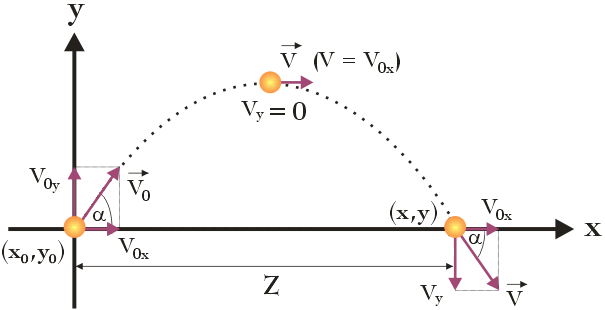
\includegraphics[width=0.7\textwidth]{img/rzut_ukosny.png}
    \end{center}
    Stosując podstawowe zależności trygonometryczne możemy rozłożyć wektor prędkości początkowej
    \[v_{x0} = v_0\cos(\alpha)\]
    \[v_{y0} = v_0\sin(\alpha)\]
    Ponieważ ciało zostało rzucone swobodnie i zaniedbujemy opory ruchu w kierunku poziomym ciało 
    porusza się ruchem jednostajnym prostoliniowym, a w kierunku pionowym jednostajnie opóźnionym 
    (później przyspieszonym) wynikającym z siły grawitacji, \textbf{wektor przyspieszenia grawitacyjnego 
    skierowany jest przeciwnie do wektora składowego prędkości początkowej w kierunku pionowym, więc 
    $g$ idzie ze znakiem $-$}:
    \[v_x = v_{x0} = v_0\cos(\alpha)\]
    \[v_y = v_{y0} - gt = v_0\sin(\alpha) - gt\]
    Teraz stosując twierdzenie pitagorasa możemy wyprowadzić zależność na prędkość \textbf{styczną do toru ruchu} od czasu:
    \[v(t) = \sqrt{v_x^2(t) + v_y^2(t)} = \sqrt{v_0 - 2v_0gtsin(\alpha) + g^2t^2}\]
    Równania ruchu względem obu osi mają następującą postać:
    \[x(t) = x_0(=0) + v_{x0}t = v_0\cos(\alpha)t\]
    \[y(t) = y_0(=0) + v_{y0}t - \frac{gt^2}{2} = v_0\sin(\alpha)t - \frac{gt^2}{2}\]
    Mając równania ruchu bardzo łatwo wyprowadzić zależnośc $y(x)$ pokazującą tor ruchu ciała:
    \[x = v_0\cos(\alpha)t \quad\implies\quad t = \frac{x}{v_0\cos(\alpha)}\]
    
    \noindent Podstawiając do równania $y(t)$ otrzymujemy:
    
    \[y(x) = v_0\sin(\alpha)\frac{x}{v_0\cos(\alpha)} - \frac{g(\frac{x}{v_0\cos(\alpha)})^2}{2}\]

    \noindent upraszczając:

    \[y(x) = x\tan{\alpha} - \frac{g}{2v_0^2\cos^2(\alpha)}x^2\]

    \noindent Aby policzyć zasięg rzutu ukośnego potrzebujemy policzyć całkowity czas wznoszenia $t_1$ i opadania $t_2$.
    Można zauważyć, że pomijając opory ruchu czasy te będą sobie równe, a więc:
    \[v_y(t_1) = 0\]
    \[v_0\sin(\alpha) - gt_1 = 0\]
    \[t_1 = \frac{v_0\sin(\alpha)}{g}\]
    \[t_c = t_1 + t_2 = 2t_1\]
    \[t_c = \frac{2v_0\sin(\alpha)}{g} \]
    Skoro mamy czas po jakim czasie ciało uderzy o ziemię, zasięg rzutu będzie równy odległości jaką ciało 
    przebędzie w kierunku poziomym:
    \[z = x(t_c) = v_0\cos(\alpha)t_c = v_0\cos(\alpha)\frac{2v_0\sin(\alpha)}{g}
    \implies z = \frac{2v_0^2\sin(2\alpha)}{g}\]

    \subsection{\LARGE Ruch po okręgu}
    \begin{definition}[Ruch po okręgu]
        Ruch w którym tor ruchu jest okrąg. Wektor prędkości $v_s$ jest stycznyczny do okręgu. 
        Występuje przyspieszenie radialne/normalne prostopadłe do wektora prędkości - oznaczamy $a_r$ 
        - gdy mówimy dokładnie o okręgu przyspieszenie to można nazwać przyspieszeniem dośrodkowym, lecz nazwać
        radialne/normalne jest bardziej ogólna.
    \end{definition}

    Aby wyprowadzić zależności opisujące ruch po okręgu rozważmy chwilię
    gdy ciało znajduje się w punkcie $P$. Przyjmuję następujące oznaczenia:
    \begin{itemize}
        \item [--] $x_P$ i $y_P$ współrzędne $x$ i $y$ punktu $P$
        \item [--] $\vec{v}$ wektor prędkości stycznej do okręgu, $v$ wartość wektora prędkości
        \item [--] $v_x$ i $v_y$ pozioma i pionowa składowa wektora prędkości $\vec{v}$
        \item [--] $r$ promień okręgu po którym odbywa się ruch
        \item [--] $\theta$ kąt pomiędzy osią $OX$ a promieniem poprowadzonym między punktami $(0,\ 0)$ i $P$
    \end{itemize}
    \begin{figure}[H]
        \centering
        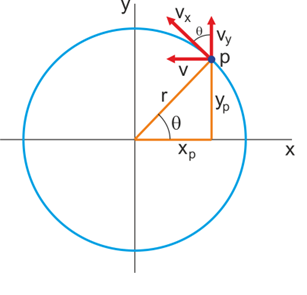
\includegraphics[]{img/ruchokrag.png}
        \caption{Na rysunku pomylono $\vec{v_x}$ i $\vec{v}$}
    \end{figure}
    Zapisujemy równania zależności trygonometrycznych:
    \[\sin\theta = \frac{y_P}{r} \quad\quad \cos\theta = \frac{x_P}{r}\]
    Rozkładamy prędkość styczną na składowe (składowa pozioma jest ujemna bo ciało porusza się "wstecz" osi $OX$):
    \[\vec{v} = \hat{i}v_x + \hat{j}v_y = \hat{i}(-v \sin\theta) + \hat{j}(v\cos\theta)\]
    \[\vec{v} = \hat{i}\left (-v \frac{y_P}{r} \right ) + \hat{j}\left (v \frac{x_P}{r} \right )\]    
    Aby obliczyć przyspieszenie "dośrodkowe" wystarczy policzyć pochodną. $v$ i $r$ to stałe więc wystarczy 
    policzyć pochodne $x_P(t)$ i $y_P(t)$.
    \[\vec{a_r} = \frac{d\vec{v}}{dt} =
    \hat{i}\left (-\frac{v}{r} \frac{dy_P}{dt} \right ) + \hat{j}\left (\frac{v}{r} \frac{dx_P}{dt} \right ) 
    = \hat{i}\left (-\frac{v}{r} v_y \right ) + \hat{j}\left (\frac{v}{r} v_x \right ) \]
    Wstawiając wzory na prędkość otrzymujemy:
    \[\vec{a_r} = \hat{i}\left (-\frac{v^2}{r} \cos\theta \right ) + \hat{j}\left (\frac{v^2}{r} \sin\theta \right )\]
    Wartość przyspiesznenia otrzymujemy z tw. Pitagorasa:
    \[a_r = \sqrt{\left (-\frac{v^2}{r} \cos\theta \right )^2 + \left (\frac{v^2}{r} \sin\theta \right )^2} = \sqrt{\frac{v^4}{r^2}(\cos^2\theta + \sin^2\theta)} = \frac{v^2}{r}\]
    Przyspieszenie radialne jest zwrócone prostopadle do toru ruchu czyli w tym wypadku do 
    środka okręgu. 

    Prędkość styczną w ruchu po okręgu możemy wyrazić korzystając z okresu ruchu $T$.
    Jeśli pokonanie całego okręgu o długości $l = 2\pi r$ zajmuje ciału czas $t_0$ to czas
    ten nazywmay okresem i oznaczmay $T = t_0$ - oznacza to czas potrzeby na pokonanie \textbf 
    jednego okręgu.
    Wtedy prędkość $v$ możemy wyrazić wzorem:
    \[v = \frac{l}{T} = \frac{2\pi r}{T} \]
    Korzystając z tego wzoru możemy wyrazić przyspieszenie dośrodkowe:
    \[a_r = \frac{v^2}{r} = \frac{\left (\frac{2\pi r}{T} \right )^2}{r} = \frac{4\pi^2 r}{T^2}\]
    Przy ruchu po okręgu/ruchu obrotowym pojawiają się wielkości skalarne opisujące stricte obrót. 
    Są to wielkości \textbf{skalarne}. Na potrzeby przyjmę następujące oznaczenia:
    \begin{itemize}
        \item [--] $s$ - długość łuku jakie zatoczyło ciało
        \item [--] $x$ i $y$ - pozycja ciała względem osi układu współrzędnych
        \item [--] $\vec{R}$ - wektor położenia względem środka układu współrzędnych, $R$ jego wartość
        \item [--] $\varphi$ - kąt jaki zatoczyło ciało
    \end{itemize}
    \begin{center}
        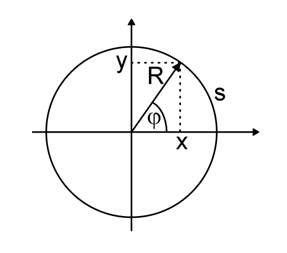
\includegraphics{img/ruchokrag2.png}
    \end{center}
    \begin{definition}[Droga kątowa]
        Jest to kąt jaki zatoczyło ciało. Jest to iloraz długości łuku przebytego przez ciało i 
        promienia wodzącego. Wyrażamy w radianach.
        \[\varphi = \frac{s(t)}{R}\]
    \end{definition}
    \begin{definition}[Prędkość kątowa]
        Jest to szybkość zmiany "kąta zatoczonego przez ciało". Analogicznie do zwykłej prędkości jest to 
        iloraz drogi kątowej przebytej w czasie. Jednostka: $\frac{1}{s}$
        \[\omega = \frac{d\varphi}{dt} = \frac{d}{dt} \frac{s(t)}{R} = \frac{v}{R}\]
        Gdy prędkość styczna jest stała, szybkość kontowa wyraża się następująco:
        \[\omega = \frac{2\pi}{T}\]
    \end{definition}
    \begin{definition}[Przyspieszenie kątowa]
        Opisuje jak zmienia się prędkość kątowa w czasie. Analogicznie do przyspieszenia w ruchu
        postępowym(zwykłym) jest to pochodna z prędkości kątowej. Jednostka $\frac{1}{s^2}$
        \[\alpha = \frac{d \omega}{dt} = \frac{d}{dt}\frac{v}{R} = \frac{a}{R} \]
    \end{definition}
    Używając tych symboli możemy wyznaczyć wzory na podstawowe wielkości opisujące ruch po okręgu.\\
    \textbf{Dla stałej prędkości stycznej:}    
    \[v = \frac{2\pi R}{T} = \omega R\]
    \[a_r = \frac{4\pi^2 R}{T^2} = \omega^2 R\]
    \textbf{Uogólnienie:}\\
    Korzystając z poprzednego rysunku równania ruchu wyglądają następująco:
    \[x(t) = R\cos \varphi(t) \quad\qquad y(t) = R\sin \varphi(t) \quad\qquad \text{gdzie: } \varphi(t) = \frac{s(t)}{R}\]
    Możemy policzyć równania prędkości:
    \[v_x = \frac{dx}{dt} = -R \frac{d\varphi}{dt}\sin \varphi = -R \omega \sin \varphi(t) \]
    \[v_y = \frac{dy}{dt} = R \frac{d\varphi}{dt}\cos \varphi = -R \omega \cos \varphi(t) \]
    Teraz przyspieszenie:
    \[a_x = \frac{d v_x}{dt} = -R \frac{d \omega}{dt} \sin \varphi - R\omega \frac{d \varphi}{dt} \cos \varphi = 
    -R\alpha \sin \varphi - R\omega^2\cos \varphi \]
    \[a_y = \frac{d v_y}{dt} = R \frac{d \omega}{dt} \cos \varphi - R\omega \frac{d \varphi}{dt} \sin \varphi = 
    R\alpha \cos \varphi - R\omega^2\sin \varphi \]
    Wstawiając równania prędkości i położenia:
    \[a_x = -R\alpha \sin \varphi - R\omega^2\cos \varphi = \frac{\alpha}{\omega}v_x - x\omega^2\]
    \[a_y = R\alpha \cos \varphi - R\omega^2\sin \varphi = \frac{\alpha}{\omega}v_y - y\omega^2\]
    Przechodząc do równania wektorowego:
    \[\vec{a} = \hat{i}a_x + \hat{j}a_y = \hat{i} \left(\frac{\alpha}{\omega}v_x - x\omega^2 \right) 
    + \hat{j} \left(  \frac{\alpha}{\omega}v_y - y\omega^2 \right) = \]
    \[= \frac{\alpha}{\omega} \left( \hat{i}v_x + \hat{j}v_y \right) - \omega^2\left( \hat{i}x + \hat{j}y \right) \]
    \[\vec{a} = \frac{\alpha}{\omega}\vec{v} -\omega^2\vec{R}\]
    W ten sposób wyprowadziliśmy wózór na wypadkowy wektor przyspieszenia w ruchu po okręgu.
    \[\vec{a} = \vec{a_s} + \vec{a_n} = \frac{\alpha}{\omega}\vec{v} -\omega^2\vec{R}\]
    \begin{center}
        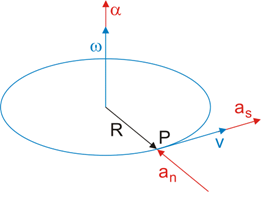
\includegraphics{img/ruchokrag3.png}
    \end{center}
    Na powyższym rysunku zaznaczono też "wektory" prędkości kątowej $\omega$ i przyspieszenia kątowego $\alpha$
    lecz wciąż należy pamiętać, że nie są to właściwe wektory, a raczej zwyczajowe oznaczenie na rysunku 
    w którą stronę się obracamy (z zasady prawej dłoni na podstawie wektora prędkości stycznej). 
    \textbf{Są to wielkości skalarne}. 
    \pagebreak
    
    \section{\huge Dynamika}
    \subsection{\LARGE Wstęp}
    Dynamika to dział zajmujący się opisywaniem przyczyn ruchu. Istnieją 4 podstawowe oddziaływania z 
    których wynikają wszystkie inne siły:
    \begin{itemize}
        \item [--] \textbf{oddziaływanie grawitacyjne} - działa na dużą odległość i dotyczy mas ciał
        \item [--] \textbf{oddziaływanie elektromagnetyczne} - działa na dużą odlgegłość i dotyczy ładunków elektrycznych i prądu
        \item [--] \textbf{oddziaływanie jądrowe słabe} - działa na małą odległość i dotyczy atomów
        \item [--] \textbf{oddziaływania jądrowe silne} - działa na małą odległości i dotyczy cząstek jądrowych
    \end{itemize}
    
    \begin{definition}[Masa]
        Najprostszą definicją masy jest \textbf{ilość materii zawartej w ciele}. Jest to jedna z 
        pierwszych definicji masy.
        
        Newton definiował masę jako \textbf{miarę bezwładności ciała}. Ma to podłoże w 
        drugiej zasadzie dynamiki gdzie masę definiujemy jako iloraz siły i przyspieszenia.
        \[m = \frac{F}{a}\]
    \end{definition}  
    Masę jakiegość ciała możemy też odnieć do masy "wzorcowej" korzystając z zasady
    zachowania pędu. Gdy rozpędzimy ciało o masie wzorcowej do prędkości $v_0$ i zderzymy
    z ciałem o masie $m$ (tak żeby ciało $m_0$ pozostawało w spoczynku po zderzeniu) to jeśli
    zmierzymy jego prędkość $v$ to jego masa wyrażać się będzie wzorem:
    \[\mathbf{m = m_0\frac{v_0}{v}}\]
    Wyprowadza się go z zasady zachowania pędu (o tym poniżej). Skoro ciało o masie $m_0$ 
    porusza się z prędkością $v_0$ to jego pęd $p_0$ wynosi $p_0 = mv_0$. Natomiast po zderzeniu
    ciało o nieznanej masie $m$ uzyska prędkość $v$, a więc jego pęd wyniesie $p = mv$.
    Skoro mówimy o zderzeniu idealnie niesprężystym możemy przyrówać te pędy:
    \[ p = p_0\]
    \[ mv = m_0v_0\]
    \[ m = m_0 \frac{v_0}{v}\]

    \begin{definition}[Pęd]
        Pęd to iloczyn masy i prędkości. 
        \[\vec{p} = m\vec{v}\]
    \end{definition} 

    \begin{definition}[Siła]
        Siłę definiujemy jako zmianę pędu w czasie.

        \[\vec{F} = \frac{d \vec{p}}{dt} = \frac{d (m \vec{v})}{dt} = m \frac{d\vec{v}}{dt} = m \vec{a}\]
    \end{definition}
    \pagebreak
    \subsection{\LARGE Zasady dynamiki Newtona}
    \begin{definition} [Zasada 1 - \textbf{\em{Zasada bezwładności}}]
        Jeśli na ciało nie działa żadna siła lub siły działające równoważą się $\left( \vec{F_{wyp}} = \bar{0} \right)$.
        To ciało pozostaje w spoczynku lub porusza się ruchem \textbf{jednostajnym prostoliniowym}.
        
        Wynika  z niej zasada zachowania pędu:
        \begin{equation}
            \sum \vec{F} = \vec{F_{wyp}} = \bar{0} \quad \implies
            \begin{cases}
                \frac{d \vec{p}}{dt} = 0 \quad \implies \quad \vec{p} = \text{const}\\
                \implies m\vec{a} = 0 \quad \implies \quad \vec{a} = 0
            \end{cases}
        \end{equation}
    \end{definition}

    
\end{document}